\section{52 --- N-Queens II (LeetCode)}

\subsection*{Código}
\lstinputlisting{52_NQueensII.java}

\subsection*{Comprovante de aceite}
\begin{center}
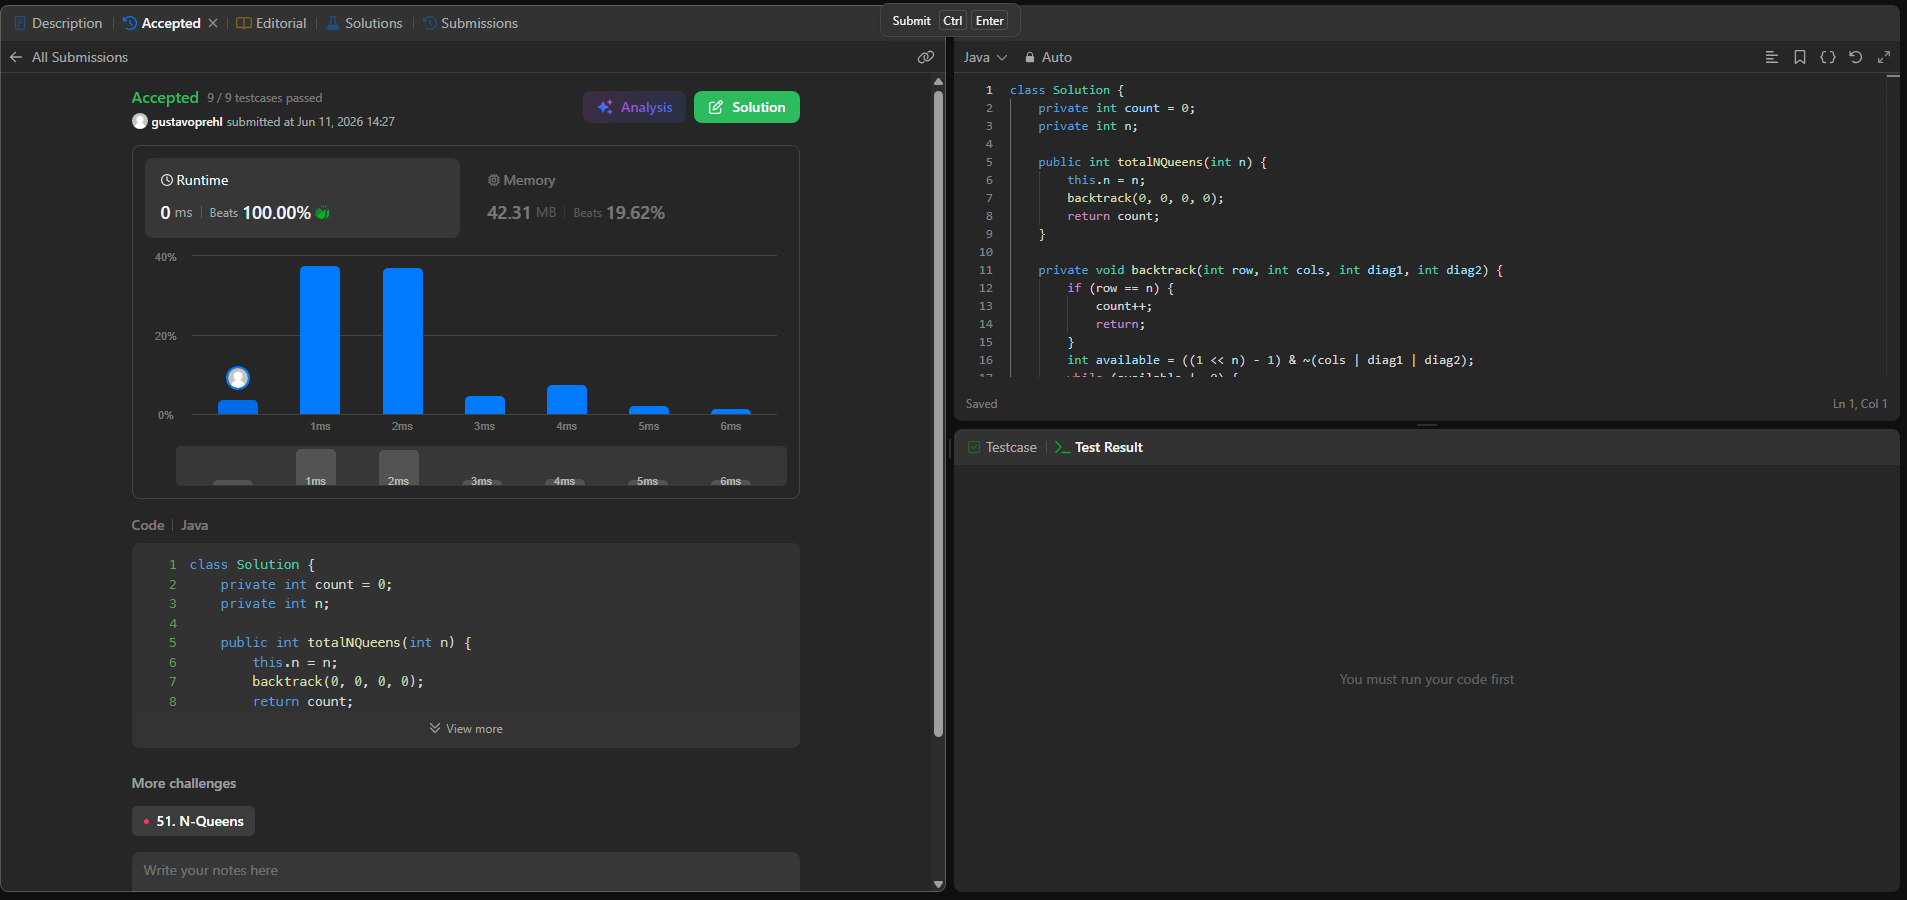
\includegraphics[width=0.85\textwidth]{Accepts/52_NQueensII_Submit.png}\\
\end{center}

\subsection*{Justificativa}

\textbf{Estratégia:} \emph{backtracking} (busca em profundidade no espaço de
soluções) com poda via \emph{bitmask}.

\textbf{Modelagem:} como duas rainhas nunca podem ficar na mesma linha, basta
decidir, para cada linha de $0$ a $n-1$, em qual coluna colocar a rainha
daquela linha. Isso reduz o espaço de busca de $2^{n^2}$ (todas as
combinações de casas) para no máximo $n^n$ (uma coluna por linha), e a poda
reduz ainda mais na prática.

\textbf{Representação por bitmask:} três inteiros guardam, em cada posição de
bit, se uma coluna (\texttt{cols}), uma diagonal principal (\texttt{diag1})
ou uma diagonal secundária (\texttt{diag2}) já está ``sob ataque'' pelas
rainhas colocadas até a linha atual. A operação
\texttt{((1 << n) - 1) \& \textasciitilde(cols | diag1 | diag2)} calcula em
$O(1)$ o conjunto de colunas livres para a linha atual.

\textbf{Poda (branch and bound):} ao avançar para a próxima linha,
atualiza-se \texttt{cols}, \texttt{diag1} (deslocada à esquerda) e
\texttt{diag2} (deslocada à direita) para refletir as novas casas atacadas.
Se, em alguma linha, \texttt{available == 0}, o ramo é descartado
imediatamente --- não há necessidade de continuar explorando colocações que
já violam as restrições do problema. Quando \texttt{row == n}, uma solução
válida completa foi encontrada e o contador é incrementado.

\textbf{Complexidade:}
\begin{itemize}
    \item Tempo: no pior caso $O(N!)$, mas a poda elimina a grande maioria
    dos ramos inválidos antes de chegar às últimas linhas (na prática, muito
    mais rápido que a enumeração ingênua).
    \item Espaço: $O(N)$ para a profundidade da recursão (não há estruturas
    adicionais de tamanho $O(N^2)$).
\end{itemize}

\textbf{Tópico do curso:} \emph{Branch-and-Bound e Backtracking} --- a busca
explora o espaço de soluções por profundidade e poda ramos inviáveis assim
que a inconsistência é detectada (\texttt{available == 0}), sem necessidade
de explorá-los até o fim.
